\documentclass[11pt,twocolumn]{article}
\usepackage[utf8]{inputenc} 
\usepackage[usenames,dvipsnames]{xcolor}
\usepackage{times}
\usepackage[T1]{fontenc}
\usepackage{amssymb,amsmath}
\usepackage{verbatim}
\usepackage{graphicx}
\usepackage{epstopdf}
\usepackage{url}
\usepackage{float}
\usepackage[ruled]{algorithm}
\usepackage{algorithmic}

\begin{document}
\title{CSE 592 - Project Report\\
  Heirarchical Co-clustering of Comic Series and their Instances}
\author{
  Chandra Sekhar Mallarapu\\
  Naresh Pratap Singh\\
  Nehal Bandi\\
  \texttt{cmallarapu@cs.stonybrook.eduTODO}}
\date{\today}
\maketitle
\titlepage
\tableofcontents
\listoffigures
\pagebreak

\section{Abstract}
In this Internet age, the comics that are available on the web have exploded. But there is no easy way for a user to find comics similar to what he is interested in. This motivates us to solve the problem of grouping together comics which are similar. In further discussions, we are going to expand about this and describe how we solved this problem.
\section{Introduction}
People have been using the medium of comics since a very long time. Comics were traditionally found only in newspapers and print material, for which people had to pay money. But in the present day, a number of people have started their own web based comic series. Another interesting fact is that some of the comics which are printed in newspapers are also available online. Hence, readers are looking more and more to the web for their comic needs. Now, a user who is reading some comic, is naturally interested in finding out other similar comics. We decided to solve this problem by creating group os similar comics together, as that will aid in future navigation and search. At a first glance, it feels like a tough problem, because the approach of doing image analysis doesnt feel like giving good results. Because, comic images are not standard and usually very rudimentary and do not represent real world entities faithfully. Another approach is to mine blogs, and search results to get this data. Our approach is to use the information in the transcripts to find similarities. This is a powerful approach because in most cases, the transcript contains not just the text of the comics, but also additional details describing the image, scene and setting too. Moreover, one doesn't have to do complex image analysis to understand what the comic is about. And in our opinion, its an easy and better way to understand and analyse the comic. Thus, the transcripts constitute our data samples. We can now do clustering on this data to find out groups of comics similar to each other. We can also use the comic series themselves as samples, and cluster them.  We decided to go one step ahead and do a heirarchical clustering, as that will allow to create coarse grained clusters too. Moreover, since similarity about comic instances hints at similarity between the comic series they belong to and vice versa. Hence, simultaneously clustering series and instances is a good way to solve the problem described earlier. Thus, the comic series names and individial instances from all series constitute our data samples. Obviously, the features needed will have to come from the text of the comics. Since we have the transcripts we can do linguistic analysis to find relevant features and similarity measures. Using that information clusters can be created.

Eckes, et al\cite{HCC2} have described an algorithm to do heirarchical co-clustering. A modification of this called \emph{HCC} is proposed in Jingxuan Li et al,\cite{HCC1}. We have modified this and used it in our project.

\section{Dataset}
We used a crawler to collect data for our project, which downloads the HTML from a web page. We then automated extraction of the comic transcript from the HTML text. In this manner, we collected transcripts of some popular comics. The size and distribution of our dataset is as follows:
\begin{itemize}
\item
  About 20528 documents from 9 comic series
\item
  Downloaded following comic series from OhNoRobot CITE
\begin{itemize}
\item
  Calvin And Hobbes - 3696 instances
\item
  College Roomies From Hell - 2631 instances
\item
  Diesel Sweeties - 1778 instances
\item
  Goats - 2266 instances
\item
  General Protection Fault - 3298 instances
\item
  Nukees - 889 instances
\item
  Questionable Content -  1747 instances
\item
  Sheldon - 3263 instances
  \end{itemize}
\item
Xkcd - 960 instances
Available from XKCD CITE
\item
  Calvin and Hobbes from blah
\end{itemize}

\section{Heirarchical Co-clustering}
We use the fact that information about documents from different series tells us about similarity between the series and vice versa. Document clustering induces series clustering while series clustering induces document clustering.
Given two types of data objects $A={a_1,a_2,\ldots,a_n}$ and $B={b_1,b_2,\ldots,b_n}$ and a matrix $X$, such that $x_{ij} \in \mathbb{R}$ represents the relation between $a_i$ and $b_j$. We need to simultaneously cluster objects in $A$ and $B$, and create heirarchies out of those clusters.
Here we describe 
HCC starts off with singleton clusters containing a tuple, which is a pair of a single document and a single series, and combines nearest two clusters in each iteration, until there is only one cluster. Thus, a dendrogram is generated, with the leaves being tuples containing a single document and a single series, and internal nodes containing a cluster of such tuples. At the root, we have all such tuples.
The HCC algorithm as given in blah is described below with a slight modification.
\begin{algorithm}[H]
  \caption{HCC Algorithm Description}
  \label{hcc_algo}
  \begin{algorithmic}
    \STATE {Create an empty heirarchy $H$}
    \STATE {$List \leftarrow$ Objects in $A$ $X$ $B$}
    \STATE {$N \leftarrow A$ $X$ $B$}
    \FOR{$i=0$ to $N-1$}
    \STATE {$p,q$=PickUpTwoNodes($List$)}
    \STATE {$o$=Merge($p,q$)}
    \STATE {Remove $p,q$ from $List$ and add $o$ to $List$}
    \STATE {Add $List$ to $H$ as next layer}
    \ENDFOR
  \end{algorithmic}
\end{algorithm}
The main step in this algorithm is which two nodes have to be merged. They are obtained in this manner.
Given a cluster $C$ with $m$ tuples, the cluster heterogenity of this cluster $CH(C)$ is defined as:
\begin{displaymath}
  CH(C)=\frac{1}{|C|}\sum_{(a_i,b_j) \in C}(x_{ij}-\mu)^2
\end{displaymath}
where $\mu=\frac{1}{|C|}\sum_{(a_i,b_j) \in C}x_{ij}$.
Another choice for $\mu$ was given in \cite{HCC2} in which they used $\mu=max(x_{ij}), \forall x_{ij} \in X$. We ran our experiment using this measure too.
The clusters to be merged are found out by calculating $CH(C_1,C_2)$, for all pairs of clusters $C_1,C_2$ from the current clusters, and picking the one which has the minimum $CH(C)$. We are determining the variance of the newly formed cluster and picking that cluster which will have least variance.
The algorithm without modification, used a very similar technique for co-clustering. The difference is that it started off with all the documents and series as the leaves, and then grouped all documents in the two clusters picked for merging in that iteration with all series from the two clusters. Here we have relaxed that constraint by having tuple of document and series as the leaves.

\section(HCC for Comics Series and Instances)
We apply the algorithm described above to our problem of creating simultaneously a heirarchical clustering of comic series and instances.
In our case, the sets of objects we have are the comic series $S$ and comic instances from all series $D$. The only detail of the \emph{HCC} algorithm specific to our problem is the relationship matrix $X$.
We used two methods to create this matrix which are described below.
\subsection{Method 1}
We use a \emph{bag of words} approach here. We run a \emph{stemmer} CITE on the transcripts to get the stems of the words present in them. From this list of words, we remove \emph{stop words} which occur in almost all documents and do not convey information that we need about the comic.
\subsubsection{Word and document relationship}
We run HCC on the words from all the documents and the documents themselves, and use the clusters of words and documents thus generated to calculate the relation between documents and series.
The \emph{tf-idf} score of a word $w$ with respect to a document $d$ is calculated based on the corpus $C$ from which this document was taken and is defined as follows:
\begin{align*}
  D(w)&=\textrm{number of documents in the corpus having word} w\\
  freq(w)&=\textrm{frequency of word} w \textrm{in document} d\\
  tf-idf(w)&=freq(w)*\log \big(\frac{|D|}{|D(w)|})
\end{align*}
Now, let $W$ represent the set of all words $w_1,w_2,\ldots,w_n$ from all the documents. We create a single corpus out of all the documents in our dataset and calculate the \emph{tf-idf} of a word $w_i$ with respect to a document $d_j$. Lets call that value as $t(w_i)$. This value $t(w_i)$ represents the relationship between $d_j$ and $w_i$ and hence we store it as the value of $x_{ij}$ in the relationship matrix between words and documents.
Note that this clustering will take $|W|+|D|-1$ iterations, creating one cluster $C_i$ in iteration $i$, by merging two clusters $C^1_i$ and $C^2_i$

\subsubsection{Document and series relationship}
The documents and series do have relations between them. What connects them is the words in the document and the words in the series. Hence, from the clusters thus generated above by HCC for words and documents, we can determine the relationship between documents and series as follows.
\begin{itemize}
\item
  Initialise all values in the relationship matrix $X$ storing the relation between documents and series to $0$.
\item
  Let $K=|W|+|D|-1$, where $W$=set of words and $D$=set of documents
\item
  For clusters $C^1_i$ and $C^2_i$ that were merged in iteration $i$ of the HCC algorithm run previously for co-clustering words and documents,
\item
  $K=K-1$
\item
  For each document $d_i$ in $C^1_i$
  \begin{itemize}
  \item
    For each series $s_j$ that each documents in $C^2_i$ belong to,
    \begin{itemize}
    \item
      \begin{displaymath}
        x_{ij}=x_{ij}+K
      \end{displaymath}
      Do the same reversing $N1$ and $N2$
    \end{itemize}
  \end{itemize}
\end{itemize}
What we have done above is utilised the clusters of words and documents created by co-clustering, to obtain values for relationship between series and documents. And since the similarity decreases as we move up this clustering, we keep decreasing the magnitude that we keep adding to the relationship strength between the documents and series present in the word-document cluster.

\begin{algorithm}[H]
  \caption{Doc-Series Relation Generator}
  \label{doc_series}
  \begin{algorithmic}
    \STATE {For all $i$ and $j$, $x_{ij}=0$}
    \STATE {$K=|W|+|D|$, where $W$=set of words and $D$=set of documents}
    \FOR{$i=1$ to $K-1$}
    \STATE {$C_i \leftarrow $ cluster created in this iteration=PickUpTwoNodes($List$)}
    \STATE {$o$=Merge($p,q$)}
    \STATE {Remove $p,q$ from $List$ and add $o$ to $List$}
    \STATE {Add $List$ to $H$ as next layer}
    \ENDFOR
  \end{algorithmic}
\end{algorithm}

For each cluster that is generated by HCC

\subsection{Method 2}
In this case, the rows of the relationship matrix $X$ are the documents and the columns are the series $S$.
We use \emph{language models} in this method.
Language models are probabilistic way of describing a corpus of text. An \emph{ngram} is a sequence of $n$ words in a text.
Viewing all documents from a series $s_i$ as a corpus, we create a \emph{ngram} language model(LM) $nLM_i$ from that corpus, where the $n$ in $nLM_i$ denotes how many \emph{ngrams} were used for creating that model. We do this for all series in our dataset, thus creating as many LMs as the number of series.
The perplexity of a given text $t$ with respect to a language model $L$ is defined as $\sqrt[N]{\frac{1}{P(t)}}$ where $P(t)$ is the probability of $t$ with respect to the LM $L$ and $N$ is the number of words in $t$. Perplexity is a measure of how likely this text could have come from that LM. A high perplexity means that the LM was surprised by that text.
For each document $d_i$, we calculate the perplexity of this document with respect to the LM $nLM_j$ created using the series $s_j$. Let $p_{ij}$ denote this value.
Since perplexity denotes the inverse of the likelihood of the text with respect to a LM, we decided that $\frac{1}{perplexity}$ is a measure of how related a document is to a series. Thus, we store $p_{ij}$ as the value of $x_{ij}$ in the relationship matrix $X$.

\section{Results and Discussion}
Below is part of a dendrogram that was generated when we ran our algorithm on 900 documents from 9 series.
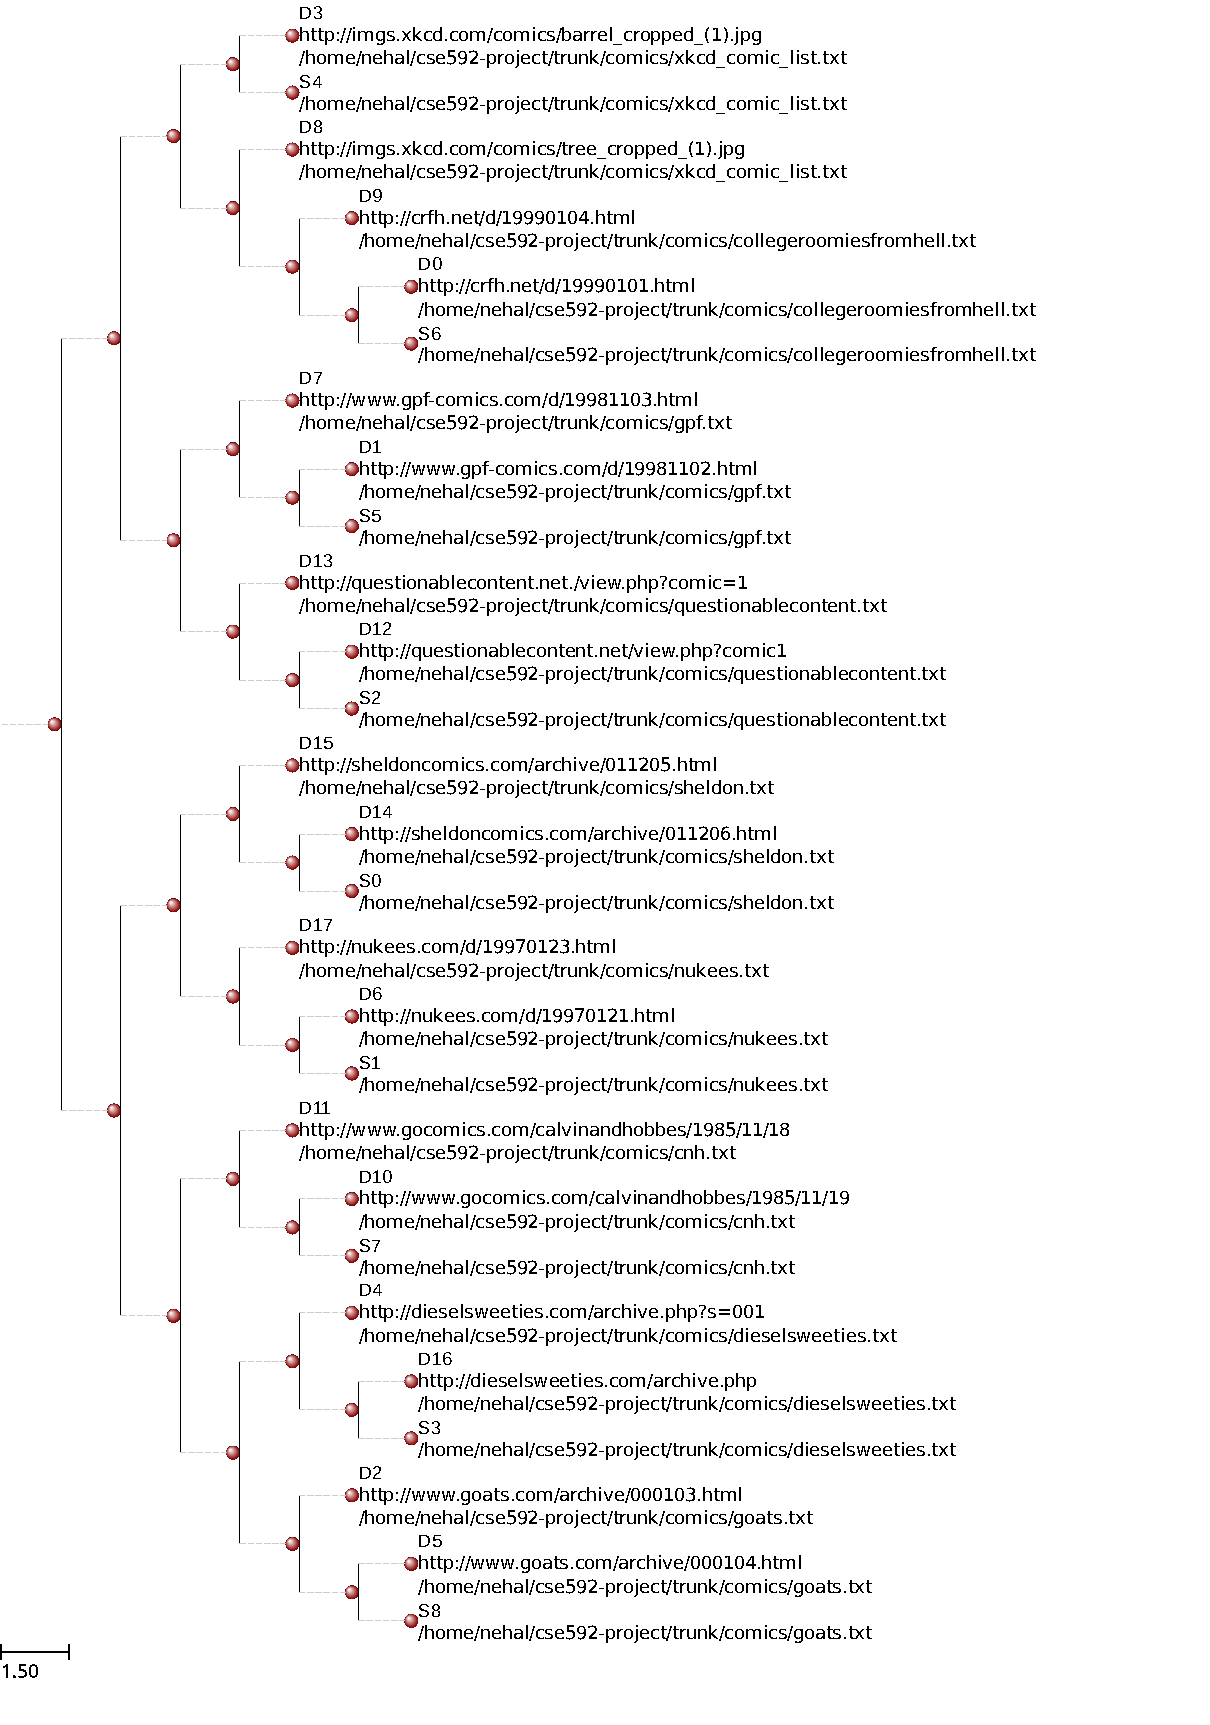
\includegraphics[height=\textheight]{demo1.pdf}
We did observe that similar comics and series were grouped together. For example, instances from series $S6$ \emph{College Roomies From Hell} were clustered with that series and then grouped with $S4$ \emph{XKCD}. We thus see a simultaneous clustering of comic series and instances.

\section{Future Work}
One area to explore is to use more sophisiticated natural language processing techniques to obtain relationship between comic series and instances. Another improvement is that once these clusters are generated, if we wanted to add in new data, the entire process has to be redone. That turns out to be quite costly and inefficient, because new data will be added frequently, as new comics are published almost every week. To solve this, we could use the current distribution of series and instances, as prior information and use sequential updating,  to determine which cluster new instances and series should be added to.
\end{document}

\begin{thebibliography}{9}
\bibitem{HCC1} Jingxuan Li et al, \emph{HCC: A Hierarchical Co-clustering Algorithm}
\bibitem{HCC2} T. Eckes et al, \emph{An error variance approach to
two-mode hierarchical clustering}
\bibitem{robot} OhNoRobot \emph{http://OhNoRobot.com}
\bibitem{xkcd} XKCD comics \emph{http://xkcd.com}
\end{thebibliography}
